%%%%%%%%%%%%%%%%%%%%%%%%%%%%%%%%%%%%%%%%%%%%%%%%%%%%%%%%%%%%%%%%%%%%%%
%%%%%%%%%%%%%%%%%%%%%%%%%%%%%%%%%%%%%%%%%%%%%%%%%%%%%%%%%%%%%%%%%%%%%%
%%%%                   Relationship arcs
%%%%%%%%%%%%%%%%%%%%%%%%%%%%%%%%%%%%%%%%%%%%%%%%%%%%%%%%%%%%%%%%%%%%%%
%%%%%%%%%%%%%%%%%%%%%%%%%%%%%%%%%%%%%%%%%%%%%%%%%%%%%%%%%%%%%%%%%%%%%%

\section{Relationships}\label{sec:relationships}

\glyph{Relationships} are rules that decide of the existence of entity nodes, based on the existence of others. 
%In ontology parlance, they would be ``occurants''. 
\SBGNERLone{} provides two types of relationships, the statements and the influences.

%%%%%%%%%%%%%%%%%%%%%%%%%%%%%%%%%%%%%%%%%%%%%%%%%%%%%%%%%%%%%%%%%%%%%%
%%%%%%%%%%%%%%%%%%%%%%%%%%%%%%%%%%%%%%%%%%%%%%%%%%%%%%%%%%%%%%%%%%%%%%
%%%%                   Statements
%%%%%%%%%%%%%%%%%%%%%%%%%%%%%%%%%%%%%%%%%%%%%%%%%%%%%%%%%%%%%%%%%%%%%%
%%%%%%%%%%%%%%%%%%%%%%%%%%%%%%%%%%%%%%%%%%%%%%%%%%%%%%%%%%%%%%%%%%%%%%

\subsection{Statements}\label{sec:statements}

\glyph{Statements} can be true or false. \glyph{Statements} are targets of \glyph{Influences}. They are not true themselves, but can  carry \glyph{Outcomes} (see \sect{outcome}). \SBGNERLone{} provides three types of statements, \glyph{Assignment}, \glyph{Interaction} and \glyph{Phenotype}.

%%%%%%%%%%%%%%%%%%%%%%%%%%%%%%%%%%%%%%%%%%%%%%%%%%%%%%%%%%%%%%%%%%%%%%
%%                    Assignment
%%%%%%%%%%%%%%%%%%%%%%%%%%%%%%%%%%%%%%%%%%%%%%%%%%%%%%%%%%%%%%%%%%%%%%
%\color{blue}

\subsubsection{Glyph: \glyph{Assignment}}\label{sec:assignment}

\glyph{Assignment} is used to describe the setting of a state variable to a certain value. The assignment, represented by an harpoon arrow, goes from on or more variable values, represented by floating \glyph{state variables} to a variable identification, represented by a \glyph{state variable} attached to the entity affected by the assignment. If an \glyph{assignment} take several \glyph{state variable} values are input, there is an implicit XOR between them. Only one value can be assigned at a time. The result of an assignment is represented by \glyph{outcomes}, that is by filled dots on the arrow. The result of an \glyph{assignment} can be represented by any number of \glyph{outcomes}. In the case of more than one \glyph{state variable} values, the \glyph{outcomes} must be placed on the relevant incoming branch.

\begin{glyphDescription}
 \glyphSboTerm non-applicable
 \glyphOrigin One or more state-variables (section \sect{stateVariable}) on their own, each containing a variable value.
 \glyphTarget A state-variable (section \sect{stateVariable}) carried by a interactor (section \sect{interactors}), containing a variable identification.
 \glyphEndPoint The target extremity of an \glyph{assignment} carries an harpoon arrowhead.
 \end{glyphDescription}

\begin{figure}[H]
  \centering
  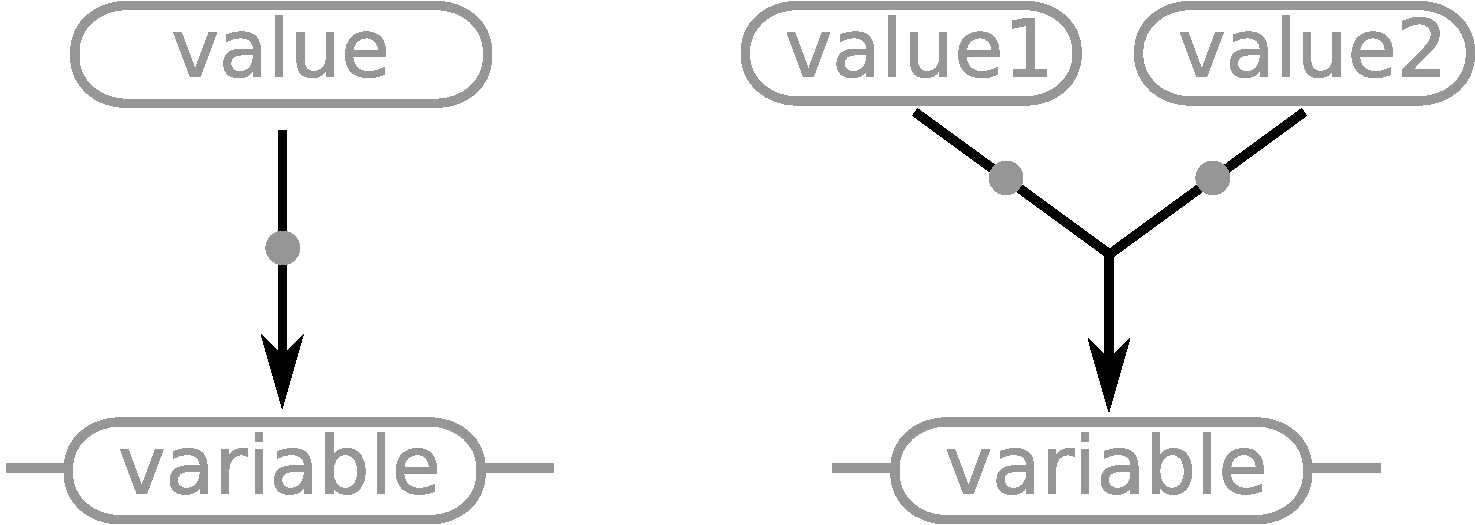
\includegraphics[scale = 0.3]{images/assignment}
  \caption{The \ER glyph for \glyph{assignment}.}
  \label{fig:assignment}
\end{figure}

\begin{figure}[H]
  \centering
  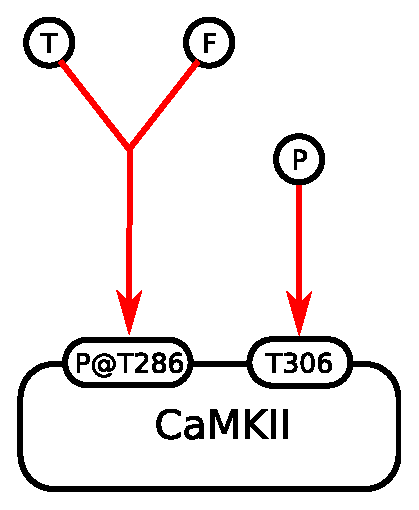
\includegraphics[scale = 0.5]{examples/ex-assignment}
  \caption{Two examples of \glyph{assignment} representing phosphorylation, by one value (phosphorylation) of a variable representing a residue, or two values (true or false) of a variable representing the phosphorylated residue.}
  \label{fig:ex-assignment}
\end{figure}


%\normalcolor

%%%%%%%%%%%%%%%%%%%%%%%%%%%%%%%%%%%%%%%%%%%%%%%%%%%%%%%%%%%%%%%%%%%%%%
%%                    Interaction
%%%%%%%%%%%%%%%%%%%%%%%%%%%%%%%%%%%%%%%%%%%%%%%%%%%%%%%%%%%%%%%%%%%%%%
%\color{blue}

\subsubsection{Glyph: \glyph{Interaction}}\label{sec:interaction}

\glyph{Interaction} represents an interaction between two or more \glyph{entities} or \glyph{outcomes}, whether a non-covalent physical interaction, or a functional interaction, e.g. genetic interaction. The interaction is represented by a circle which connect to arrows pointing to the interactors involved in the interaction. In the case of a binary interaction, the circle may be ommitted. The realisation of the interaction is represented by \glyph{outcomes} (see section \ref{sec:outcome}), that is by filled dots. These \glyph{outcomes} are located on the circle representing the interaction. In the case of a binary interaction represented without circle, the \glyph{outcomes} can be placed anywhere between the arrowheads. The realisations of an interaction can be represented by any number of \glyph{outcomes}. The \glyph{influences} (\ref{sec:influences}) targeting an interaction end up on the external side of the circle, between the \glyph{outcomes}.

\begin{glyphDescription}
 \glyphSboTerm SBO:0000342 molecular or genetic interaction
 \glyphOrigin Any \glyph{interactor} (\sect{interactors}).
 \glyphTarget Any \glyph{interactor} (\sect{interactors}).
 \glyphEndPoint Both origin and target extremities of an \glyph{interaction} carry an harpoon arrowhead. The arrows pointing to the \glyph{interactors} originate from a circle. In the case of a binary interaction, the circle is optional. 
\glyphAux A \glyph{unit of information} containing a \glyph{cardinality} (\sect{miscellaneous-cv}) indicates the number of instances of an entity involved in an interaction. The absence of a \glyph{cardinality} is synonymous of a cardinality of 1. A \glyph{unit of information} on a binary interaction involving only one entity, or outcomes of interactions involving one entity, carrying the mention \glyph{cis} or \glyph{trans} precises if the interaction is intra-molecular or between different instances of the same entity or complex.
 \end{glyphDescription}

\begin{figure}[H]
  \centering
  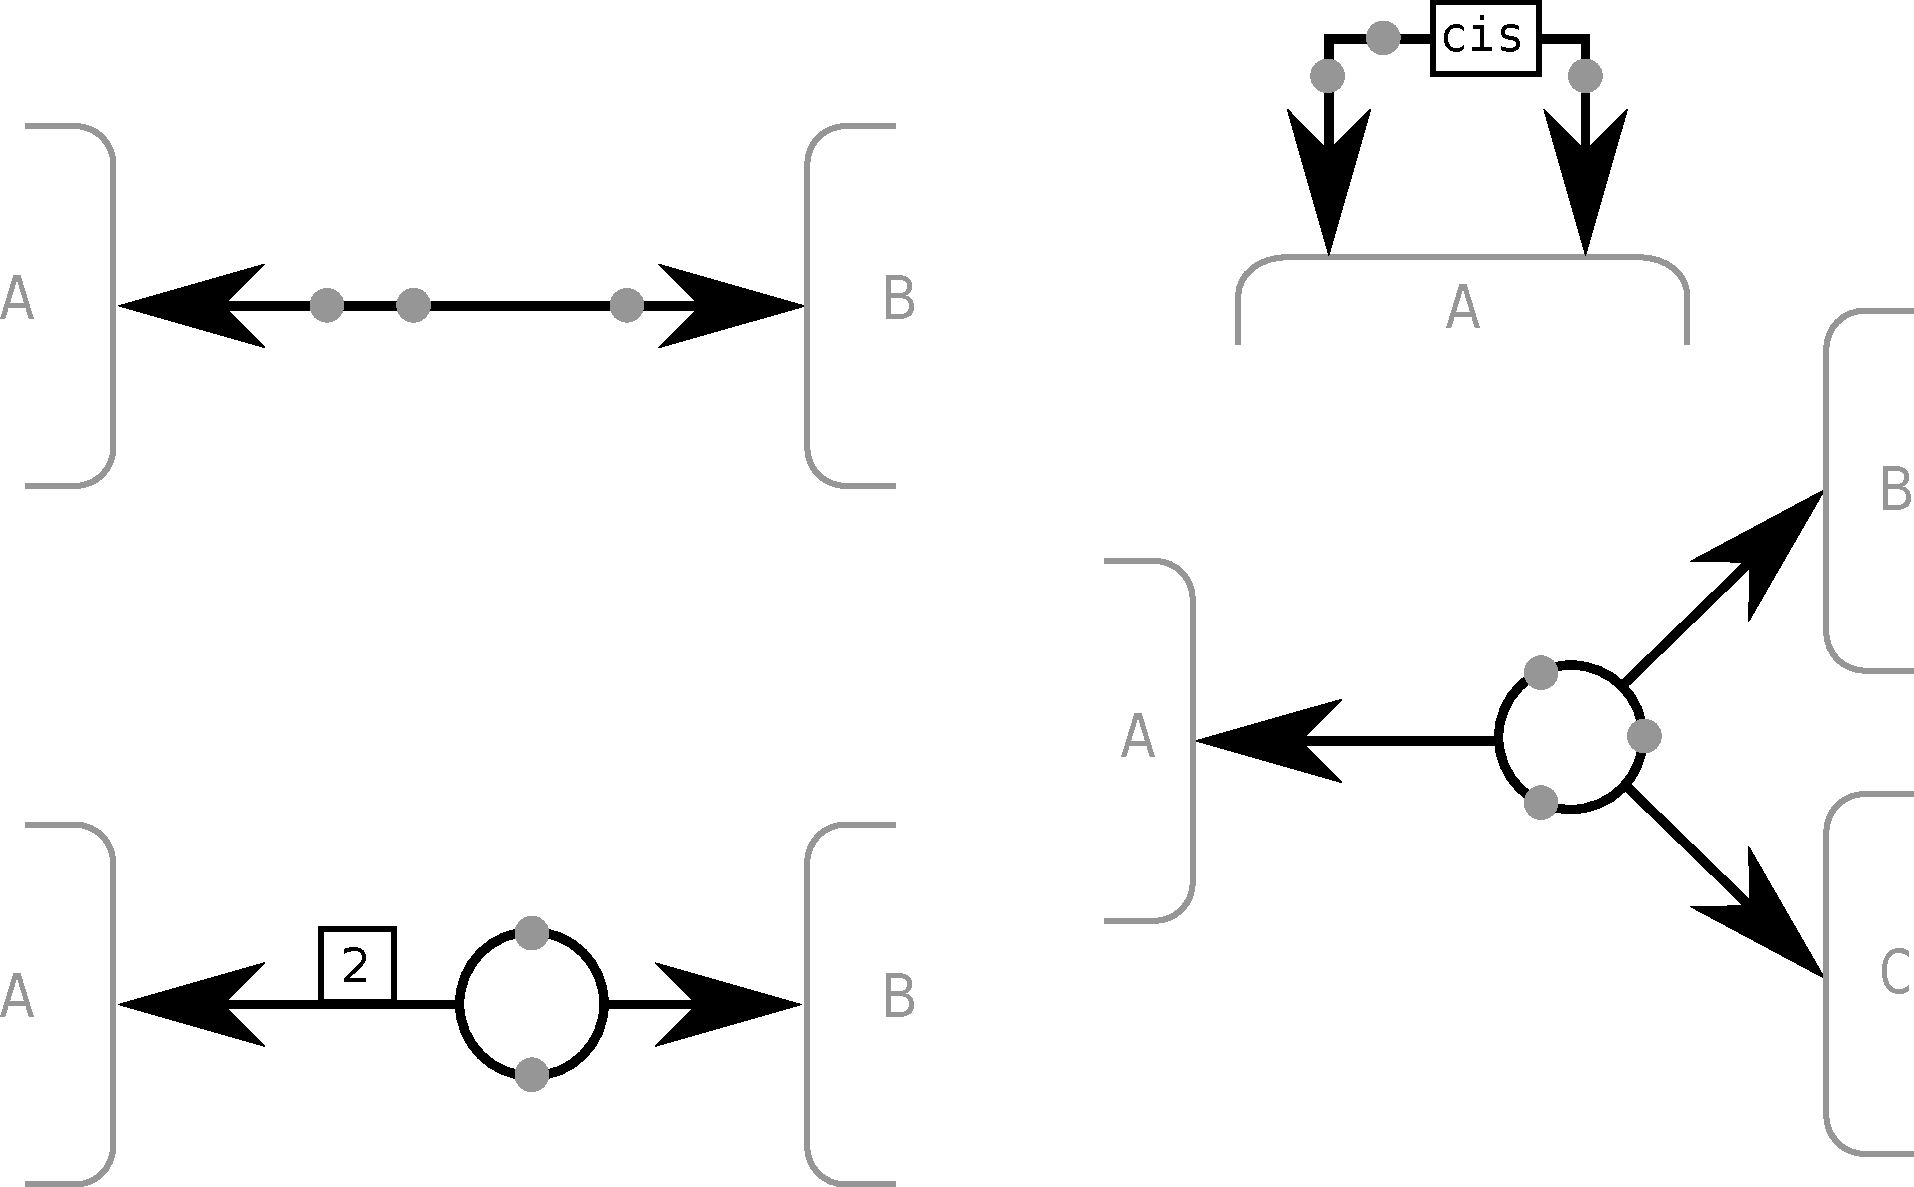
\includegraphics[scale = 0.3]{images/interaction}
  \caption{The \ER glyph for \glyph{interaction}. Top left, binary interaction between two entities. The circle can be ommitted, and the \glyph{outcomes} located anywhere on the \glyph{interaction}. Bottom left, because the cardinality of the entity A is 2, the interaction is not a binary one, but a n-ary one. The circle cannot be ommitted. Bottom right, n-ary interaction with three different entities. Top right, intra-molecular interaction; }
  \label{fig:interaction}
\end{figure}

\begin{figure}[H]
  \centering
  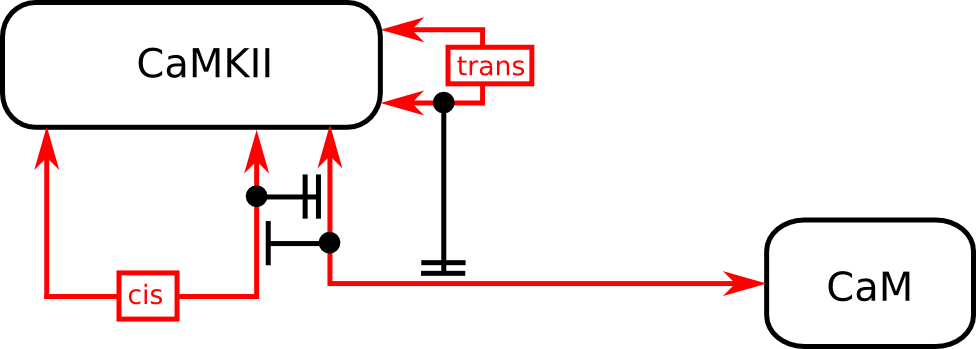
\includegraphics[scale = 0.5]{examples/ex-interaction}
  \caption{Examples of \glyph{interactions}, showing the effect of the binding of calmodulin to CaMKII (binary interaction) on the folding of the kinase (intra-molecular interaction), and the effect of the folding or the dimerisation of CaMKII (inter-molecular interaction between different instances of CaMKII) on the binding of calmodulin.}
  \label{fig:ex-interaction}
\end{figure}

\begin{figure}[H]
  \centering
  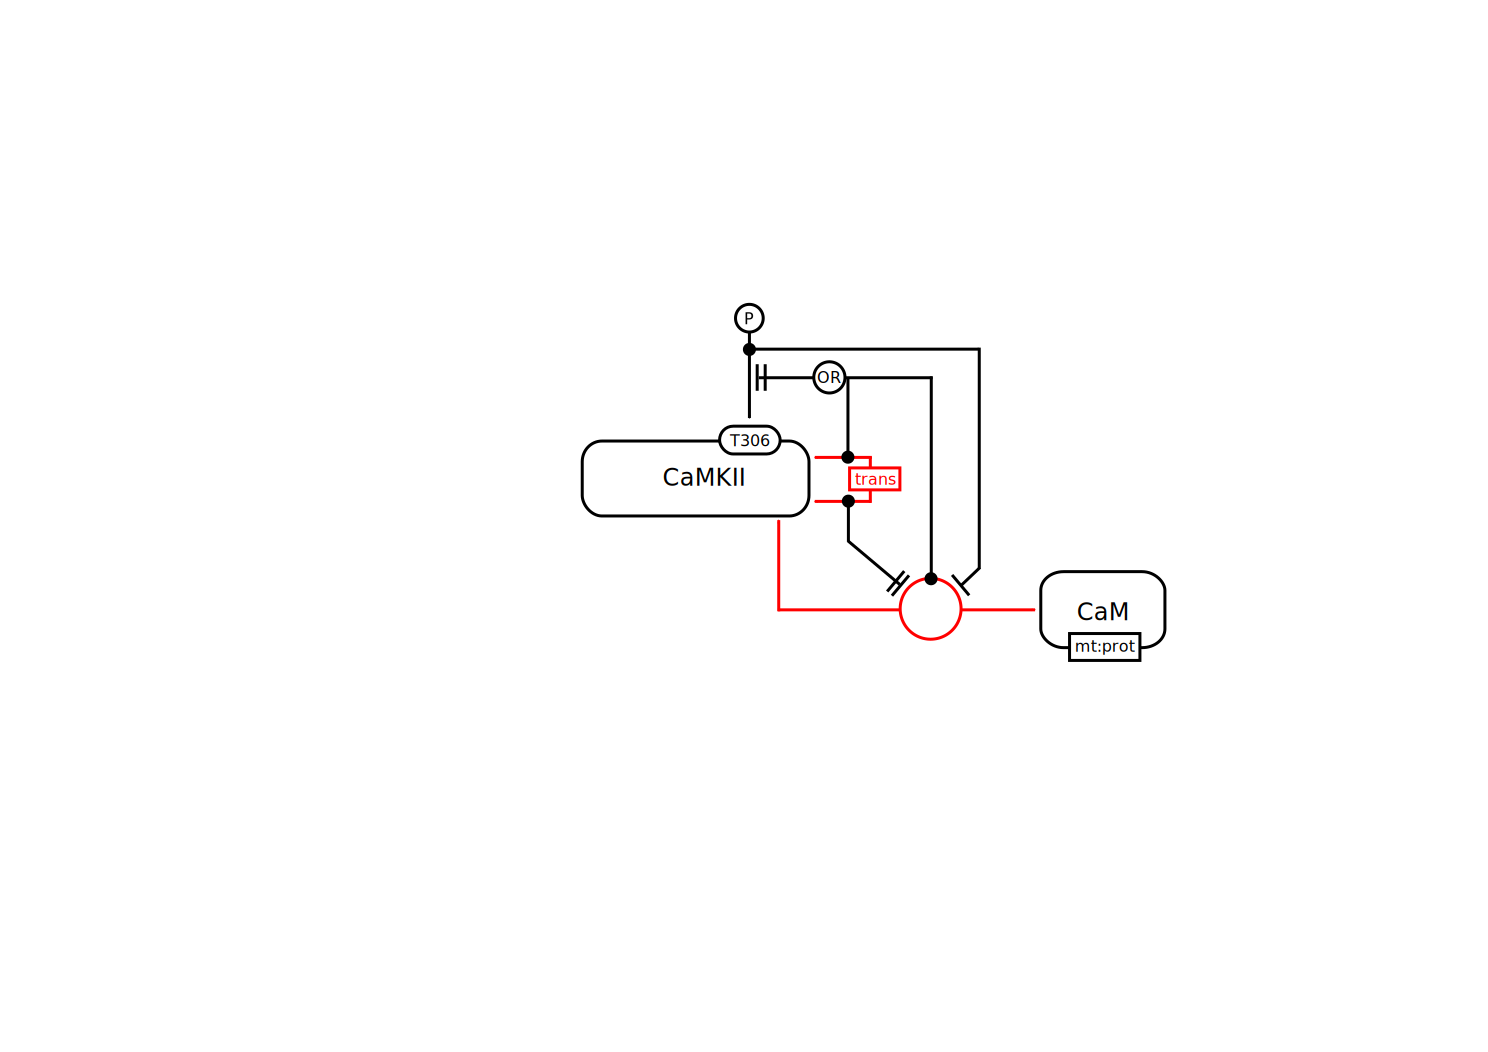
\includegraphics[scale = 0.5]{examples/ex-interaction-influences}
  \caption{Examples of a binary \glyph{interaction} between CaMKII and calmodulin where the interaction is represented by a circle. Interaction between adjacent monomers of CaMKII (trans-interaction) preclude the binding of calmodulin, as represented by an \glyph{absolute inhibition} ending on the circle. The phosphorylation of threonine 306 also inhibits the interaction. The realisation of the interaction, represented by an \glyph{outcome} located on the circle, itself inhibits the phosphorylation of threonine 306.}
  \label{fig:ex-interaction-influences}
\end{figure}
%\normalcolor

\color{ForestGreen}

\subsection{Glyph: \glyph{Phenotype}}
\label{sec:phenotype}

A biochemical network can generate phenotypes or affect biological
processes.  Such processes can take place at different levels and are
independent of the biochemical network itself.  To represent these
processes in a diagram, SBGN defines the \glyph{phenotype} glyph.

\begin{glyphDescription}

\glyphSboTerm SBO:0000358 ! phenotype
\glyphOrigin Non-applicable
\glyphTarget Non-applicable
\glyphEndPoint A \glyph{phenotype} is represented by an elongated
hexagon, as illustrated in \fig{phenotype}. It is identified by a label placed in an
unbordered box containing a string of characters.  The characters can be
distributed on several lines to improve readability, although this is not
mandatory.  The label box must be attached to the center of the
\glyph{phenotype} container.  The label may spill outside of the container.

\end{glyphDescription}
 
\begin{figure}[H]
  \centering
  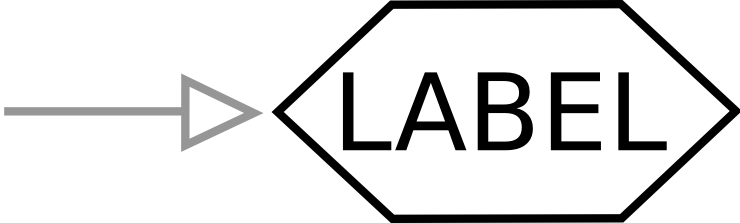
\includegraphics[scale = 0.3]{images/phenotype}
  \caption{The \ER glyph for \glyph{phenotype}.}
  \label{fig:phenotype}
\end{figure}

\begin{figure}[H]
  \centering
  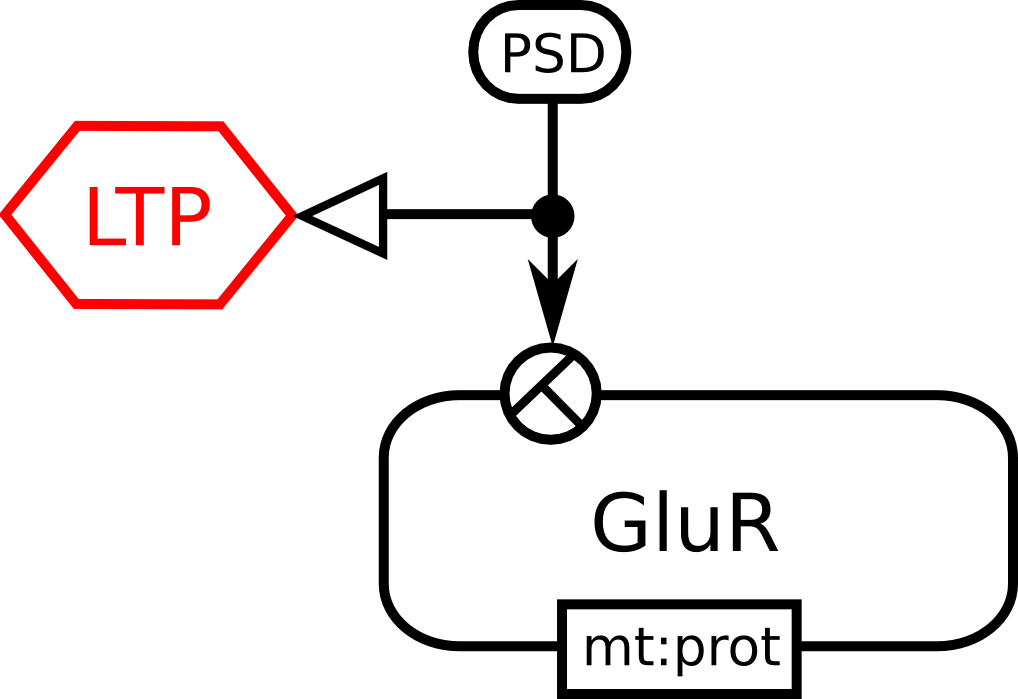
\includegraphics[scale = 0.5]{examples/ex-phenotype}
  \caption{Example of a \glyph{phenotype} ``Long Term Potentiation (LTP)'' enhanced when the entity ``GluR'' is present in the post-synaptic density.}
  \label{fig:ex-phenotype}
\end{figure}

\normalcolor


\subsection{Influences}\label{sec:influences}

Influence arcs represent the effect of an entity on another relationship. The symbols attached to their extremities precise their semantics. SBGN \ERs{}' influences can be viewed as logical rules linking \glyph{ENs} and other rules. \SBGNERLone{} provides seven influences, \glyph{Modulation}, \glyph{Stimulation}, \glyph{Inhibition}, \glyph{Necessary Stimulation}, \glyph{Absolute Inhibition}, \glyph{Absolute Stimulation}, \glyph{Logic Arc}.

%%%%%%%%%%%%%%%%%%%%%%%%%%%%%%%%%%%%%%%%%%%%%%%%%%%%%%%%%%%%%%%%%%%%%%
%%                     Modulation
%%%%%%%%%%%%%%%%%%%%%%%%%%%%%%%%%%%%%%%%%%%%%%%%%%%%%%%%%%%%%%%%%%%%%%
\color{blue}
\subsubsection{Glyph: \glyph{Modulation}}\label{sec:modulation}

A modulation affects the strength, or the probability to exist, of the target relationship. Such a modulation can affect the relationship \textbf{positively or negatively}, or even both ways depending on the conditions. A \glyph{modulation} can also be used when one does not know the precise direction of the effect, for instance if there are conflicting evidence.

\begin{glyphDescription}
 \glyphSboTerm SBO:0000168 ! control.
 \glyphOrigin Any \glyph{entity node} (\sect{ENs}).
 \glyphTarget Any \glyph{relationship} (\sect{relationships}).
 \glyphEndPoint The target extremity of a \glyph{modulation} carries an empty diamond.
 \end{glyphDescription}

\begin{figure}[H]
  \centering
  
\includegraphics[scale = 0.5]{images/modulation}
  \caption{The \ER glyph for \glyph{modulation}.}
  \label{fig:modulation}
\end{figure}
 
\begin{figure}[H]
  \centering
  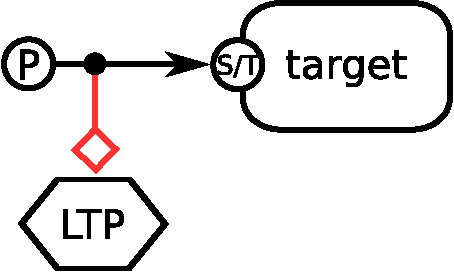
\includegraphics[scale = 0.5]{examples/ex-modulation}
  \caption{Example of a \glyph{modulation} of the \glyph{phenotype} ``Long Term Potentiation (LTP)'' by the phosphorylation of an \glyph{entity} ``target''. For instance the influence could be positive (stimulation, see \sect{stimulation}) or negative (inhibition, see \sect{inhibition}).}
  \label{fig:ex-modulation}
\end{figure}

\normalcolor


%%%%%%%%%%%%%%%%%%%%%%%%%%%%%%%%%%%%%%%%%%%%%%%%%%%%%%%%%%%%%%%%%%%%%%
%%                     Stimulation
%%%%%%%%%%%%%%%%%%%%%%%%%%%%%%%%%%%%%%%%%%%%%%%%%%%%%%%%%%%%%%%%%%%%%%

\subsubsection{Glyph: \glyph{Stimulation}}\label{sec:stimulation}
\color{blue}

A \glyph{stimulation} affects \textbf{positively} the strength, or the probability, of the target relationship. This stimulation can be for instance a catalysis or a positive allosteric regulation.

\begin{glyphDescription}
 \glyphSboTerm SBO:0000170 ! stimulation.
 \glyphOrigin Any \glyph{entity node} (\sect{ENs}).
 \glyphTarget Any \glyph{relationship} (\sect{relationships}).
 \glyphEndPoint The target extremity of a \glyph{stimulation} carries an empty arrowhead.
 \glyphAux A \glyph{unit of information} carrying the mention \glyph{cis} or \glyph{trans} precises the relationship between the \glyph{entity node} from which the \glyph{stimulation} origins and either:
\begin{itemize}
\item the \glyph{entity node} from which the influence targeted by the \glyph{stimulation} origins
\item all the relevant \glyph{interactors} of the \glyph{interaction} or the \glyph{non-interaction} targeted by the \glyph{stimulation}
\item the \glyph{entity} subjected to the \glyph{assignment} targeted by the \glyph{stimulation}
\end{itemize}
 \end{glyphDescription}

\begin{figure}[H]
  \centering
  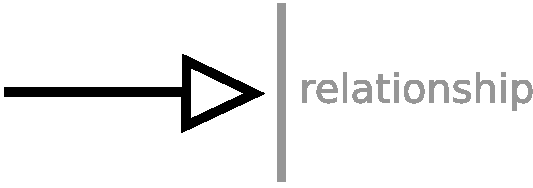
\includegraphics[scale = 0.5]{images/stimulation}
  \caption{The \PD glyph for \glyph{stimulation}.}
  \label{fig:stimulation}
\end{figure}

\begin{figure}[H]
  \centering
  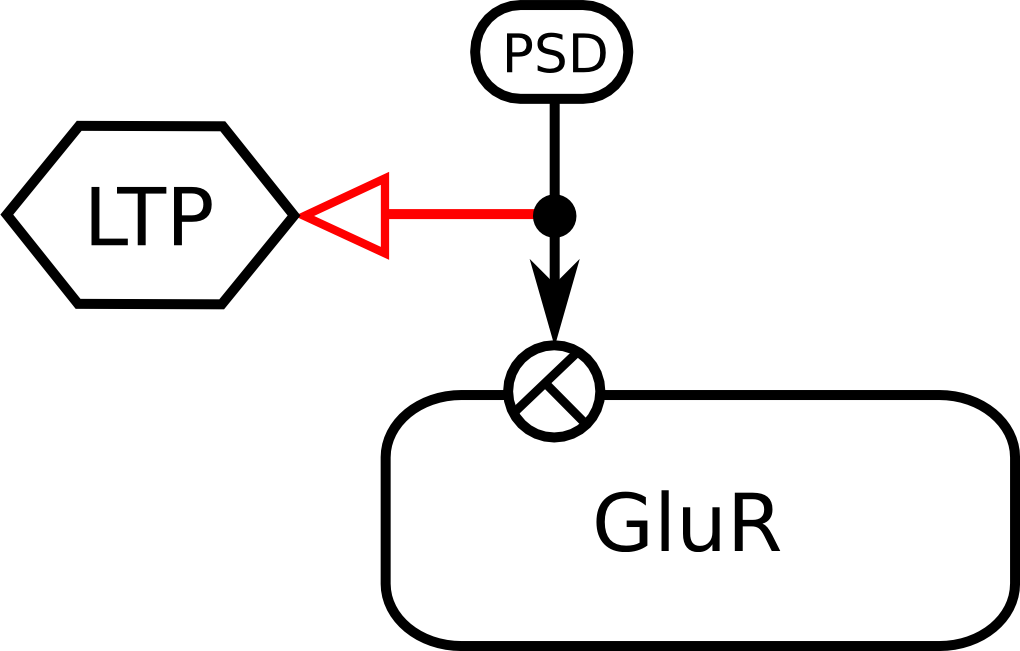
\includegraphics[scale = 0.5]{examples/ex-stimulation}
  \caption{Example of a \glyph{stimulation} a \glyph{phenotype} ``Long Term Potentiation (LTP)'' enhanced when the entity ``GluR'' is present in the post-synaptic density.}
  \label{fig:ex-stimulation}
\end{figure}

\normalcolor




%%%%%%%%%%%%%%%%%%%%%%%%%%%%%%%%%%%%%%%%%%%%%%%%%%%%%%%%%%%%%%%%%%%%%%
%%                     Inhibition
%%%%%%%%%%%%%%%%%%%%%%%%%%%%%%%%%%%%%%%%%%%%%%%%%%%%%%%%%%%%%%%%%%%%%%

\subsubsection{Glyph: \glyph{Inhibition}}\label{sec:inhibition}
\color{blue}

An inhibition \textbf{negatively}  the strength, or the probability, of the target relationship. This inhibition can be for instance a steric hindrance or a negative allosteric regulation.

\begin{glyphDescription}
 \glyphSboTerm SBO:0000170 ! inhibition.
 \glyphOrigin Any \glyph{entity node} (\sect{ENs}).
 \glyphTarget Any \glyph{relationship} (\sect{relationships}).
 \glyphEndPoint The target extremity of a \glyph{inhibition} carries a bar perpendicular to the arc.
 \end{glyphDescription}

\begin{figure}[H]
  \centering
  
\includegraphics[scale = 0.3]{images/inhibition}
  \caption{The \PD glyph for \glyph{inhibition}.}
  \label{fig:inhibition}
\end{figure}

\begin{figure}[H]
  \centering
  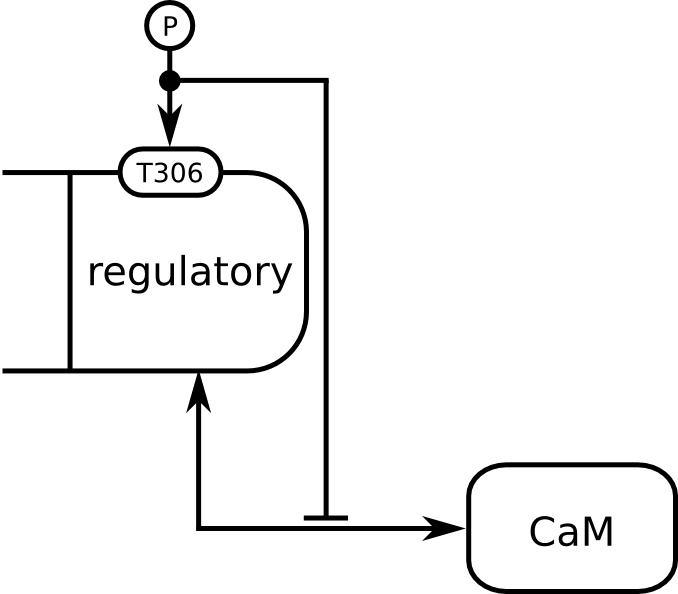
\includegraphics[scale = 0.5]{examples/ex-inhibition}
  \caption{In this example, the phosphorylation of the threonine 306 of the regulatory domain of CaMKII inhibits the interaction between Calmodulin and the kinase.}
  \label{fig:ex-inhibition}
\end{figure}

\normalcolor


%%%%%%%%%%%%%%%%%%%%%%%%%%%%%%%%%%%%%%%%%%%%%%%%%%%%%%%%%%%%%%%%%%%%%%
%%                     necessary stimulation
%%%%%%%%%%%%%%%%%%%%%%%%%%%%%%%%%%%%%%%%%%%%%%%%%%%%%%%%%%%%%%%%%%%%%%
%\color{blue}

\subsubsection{Glyph: \glyph{Necessary stimulation}}\label{sec:necessaryStimulation}

A \glyph{necessary stimulation} is an influence that has to be present for a relationship to take place (to become true). A relationship modulated by a necessary stimulation can only exist when this stimulation is true, whatever are the other influences this relationship is subjected to.

\begin{glyphDescription}
 \glyphSboTerm SBO:0000171 ! necessary stimulation.
 \glyphOrigin Any \glyph{entity node} (\sect{ENs}).
 \glyphTarget Any \glyph{relationship} (\sect{relationships}).
 \glyphEndPoint The target extremity of a \glyph{necessary stimulation} carries an open arrow (to remind that it is a \glyph{stimulation}) coming after a larger vertical bar.
 \glyphAux A \glyph{unit of information} carrying the mention \glyph{cis} or \glyph{trans} precises the relationship between the \glyph{entity node} from which the \glyph{necessary stimulation} origins and either:
\begin{itemize}
\item the \glyph{entity node} from which the influence targeted by the \glyph{necessary stimulation} origins
\item all the relevant \glyph{interactors} of the \glyph{interaction} targeted by the \glyph{necessary stimulation}
\item the \glyph{entity} subjected to the \glyph{assignment} targeted by the \glyph{necessary stimulation}
\end{itemize}

 \end{glyphDescription}

\begin{figure}[H]
  \centering
  
\includegraphics[scale = 0.5]{images/necessaryStimulation}
  \caption{The \ER glyph for \glyph{necessaryStimulation}.}
  \label{fig:necessaryStimulation}
\end{figure}

\begin{figure}[H]
  \centering
  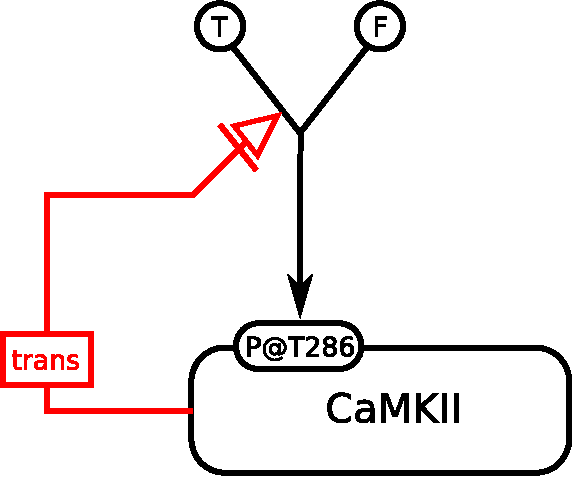
\includegraphics[scale = 0.5]{examples/ex-necessaryStimulation}
  \caption{This example shows how threonine 286 of CaMKII is only phosphorylated by the kinase itself, but in a trans-fashion, meaning a molecule of CaMKII does not phosphorylate itself, but another molecule of CaMKII.}
  \label{fig:ex-necessaryStimulation}
\end{figure}

%\normalcolor
%%%%%%%%%%%%%%%%%%%%%%%%%%%%%%%%%%%%%%%%%%%%%%%%%%%%%%%%%%%%%%%%%%%%%%
%%                     absolute stimulation
%%%%%%%%%%%%%%%%%%%%%%%%%%%%%%%%%%%%%%%%%%%%%%%%%%%%%%%%%%%%%%%%%%%%%%
\color{red}

\subsubsection{Glyph: \glyph{Absolute inhibition}}\label{sec:absoluteInhibition}

An absolute inhibition precludes the existence of another relationship. A relationship modulated by an absolute inhibition can only exist when an absolute inhibition in false, whatever are the other influences this relationship is subjected to.

\begin{glyphDescription}
 \glyphSboTerm SBO:0000171 ! absolute inhibition.
 \glyphOrigin Any \glyph{entity node} (\sect{ENs}).
 \glyphTarget Any \glyph{relationship} (\sect{relationships}).
 \glyphEndPoint The target extremity of a \glyph{absolute inhibition} carries a double bar perpendicular to the arc (to remind that it is an \glyph{inhibition}).
 \end{glyphDescription}

\begin{figure}[H]
  \centering
  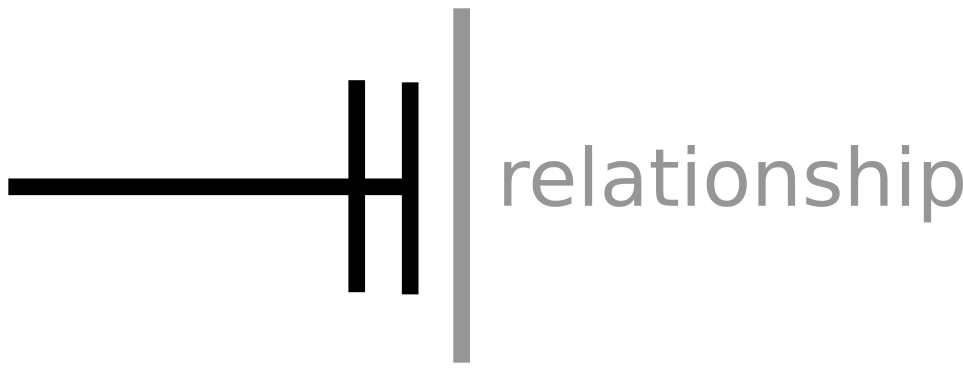
\includegraphics[scale = 0.5]{images/absoluteInhibition}
  \caption{The \PD glyph for \glyph{absoluteInhibition}.}
  \label{fig:absoluteInhibition}
\end{figure}

\begin{figure}[H]
  \centering
  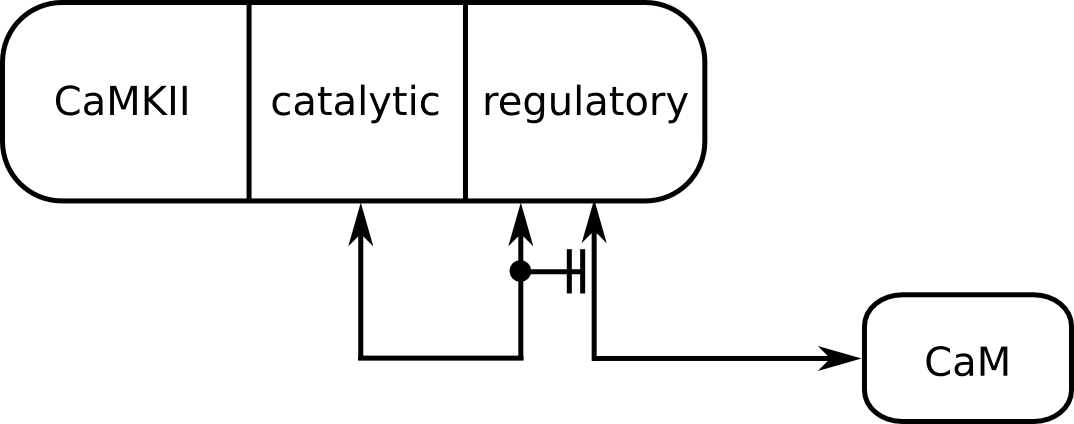
\includegraphics[scale = 0.5]{examples/ex-absoluteInhibition}
  \caption{This example shows how an intra-molecular interaction between catalytic and regulatory domains of CaMKII precludes totally the interaction of Calmodulin with CaMKII.}
  \label{fig:ex-absoluteInhibition}
\end{figure}

\normalcolor
%%%%%%%%%%%%%%%%%%%%%%%%%%%%%%%%%%%%%%%%%%%%%%%%%%%%%%%%%%%%%%%%%%%%%%
%%                     absolute stimulation
%%%%%%%%%%%%%%%%%%%%%%%%%%%%%%%%%%%%%%%%%%%%%%%%%%%%%%%%%%%%%%%%%%%%%%
\color{red}

\subsubsection{Glyph: \glyph{Absolute stimulation}}\label{sec:absoluteStimulation}

An absolute stimulation always trigger the existence of a target relationship. 

\begin{glyphDescription}
 \glyphSboTerm SBO:0000411 ! absolute stimulation
 \glyphOrigin Any \glyph{entity node} (\sect{ENs}).
 \glyphTarget Any \glyph{relationship} (\sect{relationships}).
 \glyphEndPoint The target extremity of a \glyph{absolute inhibition} carries a double empty arrowhead (to remind that it is a \glyph{stimulation}).
 \end{glyphDescription}

\begin{figure}[H]
  \centering
  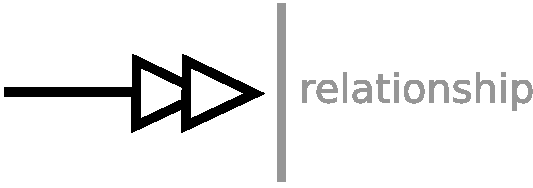
\includegraphics[scale = 0.5]{images/absoluteStimulation}
  \caption{The \PD glyph for \glyph{absoluteStimulation}.}
  \label{fig:absoluteStimulation}
\end{figure}


\normalcolor
%%%%%%%%%%%%%%%%%%%%%%%%%%%%%%%%%%%%%%%%%%%%%%%%%%%%%%%%%%%%%%%%%%%%%%
%%                     Logic arc
%%%%%%%%%%%%%%%%%%%%%%%%%%%%%%%%%%%%%%%%%%%%%%%%%%%%%%%%%%%%%%%%%%%%%%
%\color{blue}
\subsubsection{Glyph: \glyph{Logic arc} }\label{sec:logicArc}

\glyph{Logic arc} is used to represent the fact that an interactor influences
the outcome of a logic operator. 

\begin{glyphDescription}
 \glyphSboTerm SBO:0000398 - logical relationship.
 \glyphOrigin Any \glyph{interactor} (\sect{interactors}) or \glyph{logical operator} (\sect{logic}).
 \glyphTarget Any \glyph{logical operator} (\sect{logic}).
 \glyphEndPoint No particular symbol is used to represent a logic arc.
 \end{glyphDescription}

\begin{figure}[H]
  \centering
  
\includegraphics[scale = 0.4]{images/logicArc}
  \caption{The \ER glyph for \glyph{logic arc}.}
  \label{fig:logicArc}
\end{figure}

\begin{figure}[H]
  \centering
  \includegraphics[scale = 0.5]{examples/ex-logicArc}
  \caption{In this example, two logic arcs reflect the fact that the phosphorylation of threonine 306 on CaMKII is precluded either by a dimerisation or the binding of calmodulin.}
  \label{fig:ex-logicArc}
\end{figure}

%\normalcolor



%\section{Submap}\label{sec:submap}
%%%%%%%%%%%%%%%%%%%%%%%%%%%%%%%%%%%%%%%%%%%%%%%%%%%%%%%%%%%%%%%%%%%%%%%
%%%%                   Submap
%%%%%%%%%%%%%%%%%%%%%%%%%%%%%%%%%%%%%%%%%%%%%%%%%%%%%%%%%%%%%%%%%%%%%%

\color{red}

A \glyph{submap} is used to encapsulate entities and relationships (including all types of nodes and edges) within one named glyph. The content of the submap can be found for instance on another (web) page in the case of static maps, or can be displayed dynamicaly. Because of the independence of rules, no particular connections are needed between the submap and the containing map.

\begin{figure}[H]
  \centering
  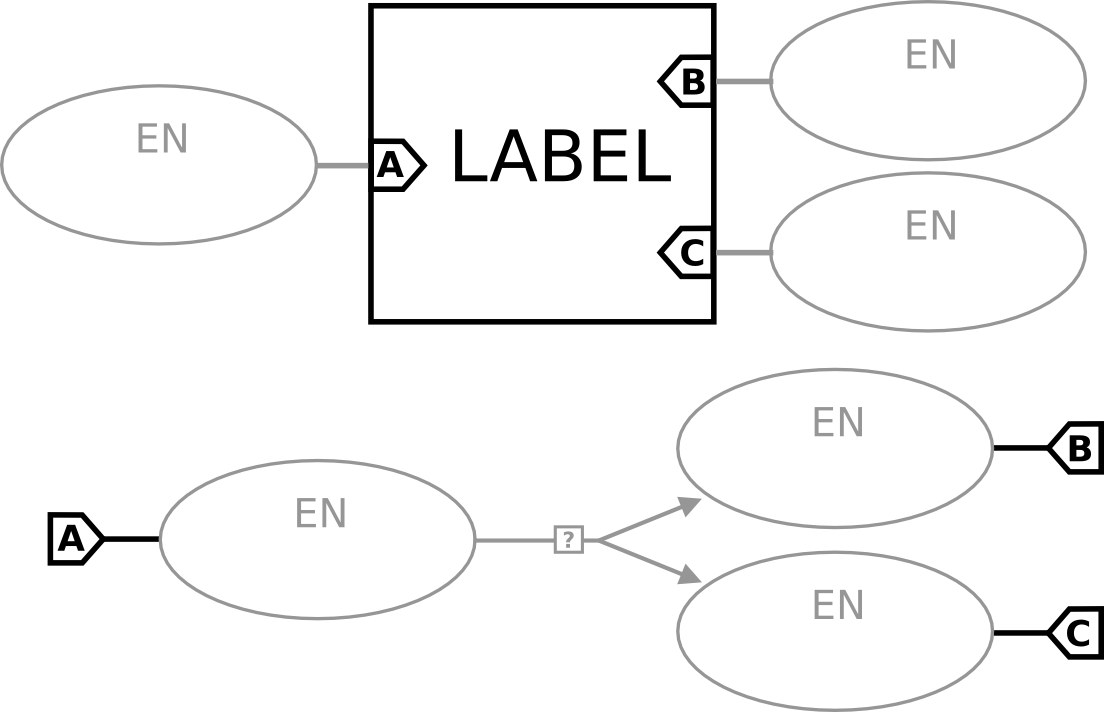
\includegraphics[scale = 0.3]{images/submap}
  \caption{The \ER glyph for \glyph{submap}.}
  \label{fig:submap}
\end{figure}


\normalcolor


